\section{ニコ書を支える命名の儀}

いろいろな人が名前大事と言っているように、ニコ書チームも命名にはとてもこだわります。
プロジェクトのスタートは、みんなでウンウン唸りながらプロジェクト名を考えます。
プロジェクト名だけでなく、新バージョンの開発コードや、新機能の通称など、
ありとあらゆる物に捻った名前をつけることに無駄にリソースを費やします。

もちろん、クラス名やメソッド名について激しい議論を交わすことも
\emph{たまに} あります。

ここでつけたプロジェクト名は、チーム内だけ通用するだけではなく、
githubのプロジェクト名として使われ、他チームとのやり取りでも使われ、
偉い人への説明などでも堂々と使われます。

一番特徴的なプロジェクト名の付け方をいくつか紹介します

\subsection{大原則}

別に誰が決めたわけではないですが、なぜか ``\emph{俺の嫁}''
の名前をつけることが大前提になっています。
本当に誰かが規則にしたわけではないのです。
どうせ名前をつけてそれを呼ぶのなら、可愛い女の子の名前を呼びたいよね・・・という心理が働いているのでしょうか。

そしてもちろん女の子の名前なので、呼ぶときはキャラに合わせて「ちゃん付け」や「さん付け」をします。
当然偉い人の前でも。

\subsection{パターン1: とにかく今の嫁!}

いきなり例外的な例ですが、何も考えずにとにかく今好きで好きでたまらない嫁の名前をつける場合があります。
すべての思考を捨て去った動物的な命名ですが、それだけ名前に強いパワーがあるような感じがします。
この命名が行われる場合は、メンバー全員が納得できるくらい
\emph{非常にメジャーな作品} か \emph{チーム内で大流行してる作品}
から取られます。

このパターンで付けられた名前は

\begin{itemize}
\itemsep1pt\parskip0pt\parsep0pt
\item
  \emph{ほむらちゃん} 外部サービス連携サーバ。もちろん『まどマギ』
\item
  \emph{まくらちゃん} iOS版ver.2の開発コード。 『パジャマな彼女』より
\item
  \emph{うまるちゃん} モバイル用サイト。YJの『干物妹 うまるちゃん』
\end{itemize}

\begin{figure}[H]
  \centering
  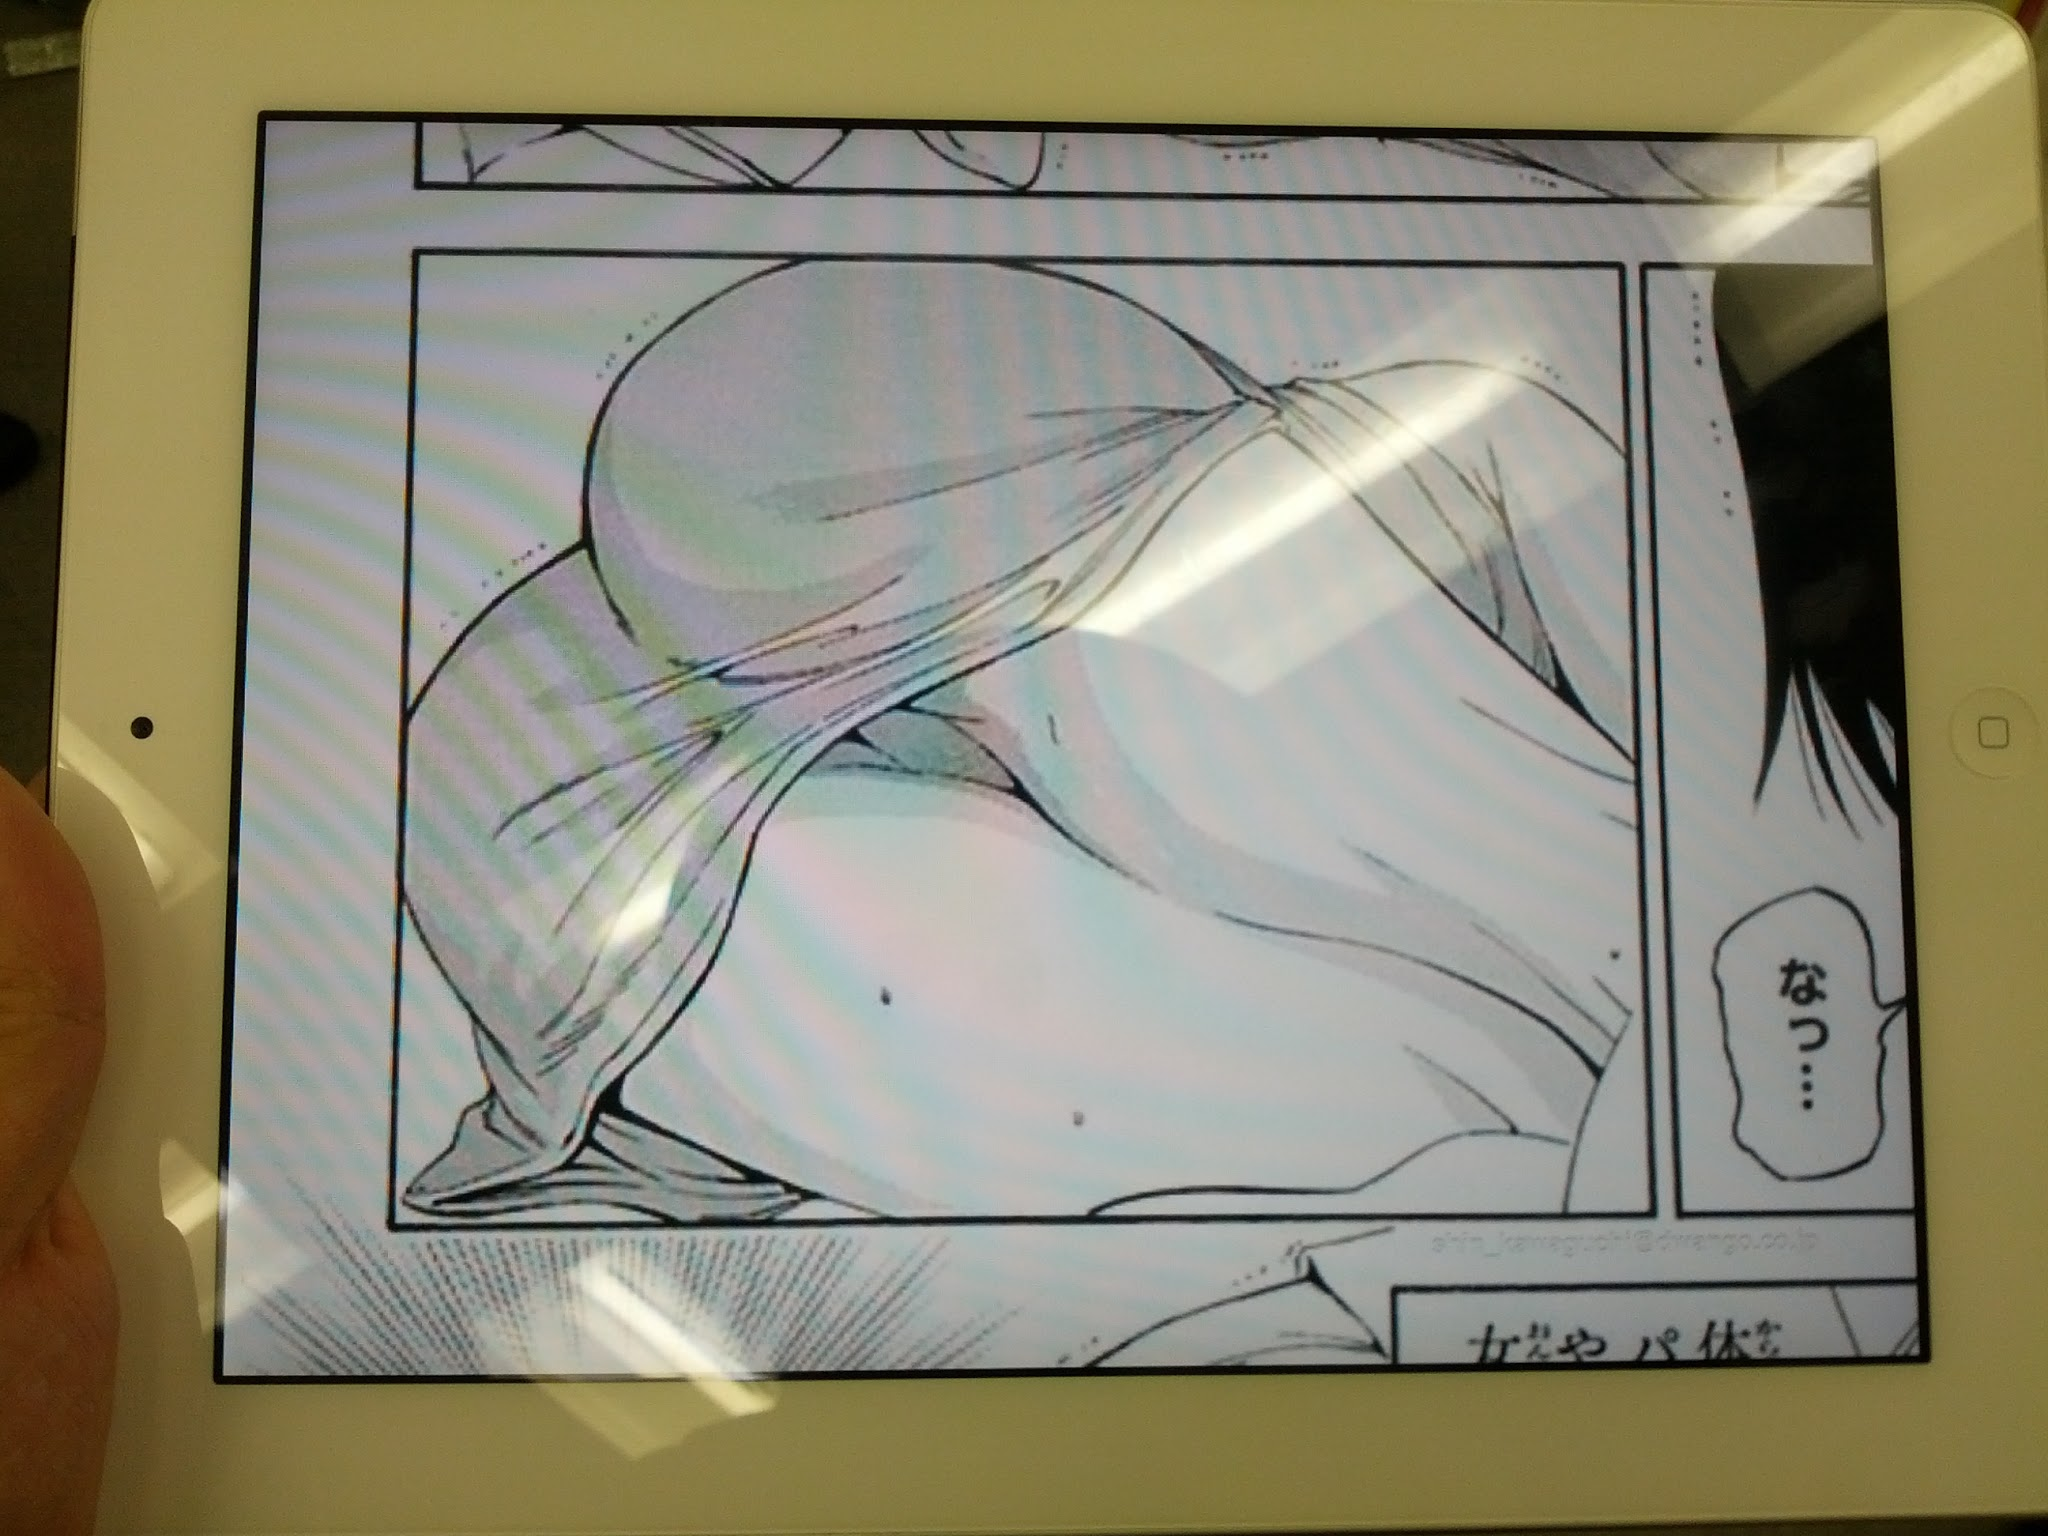
\includegraphics[width=0.4\textwidth]{../images/makura.jpg}
  \caption{まくらちゃんでまくらちゃんを表示してみる}
\end{figure}

\begin{figure}[H]
  \centering
  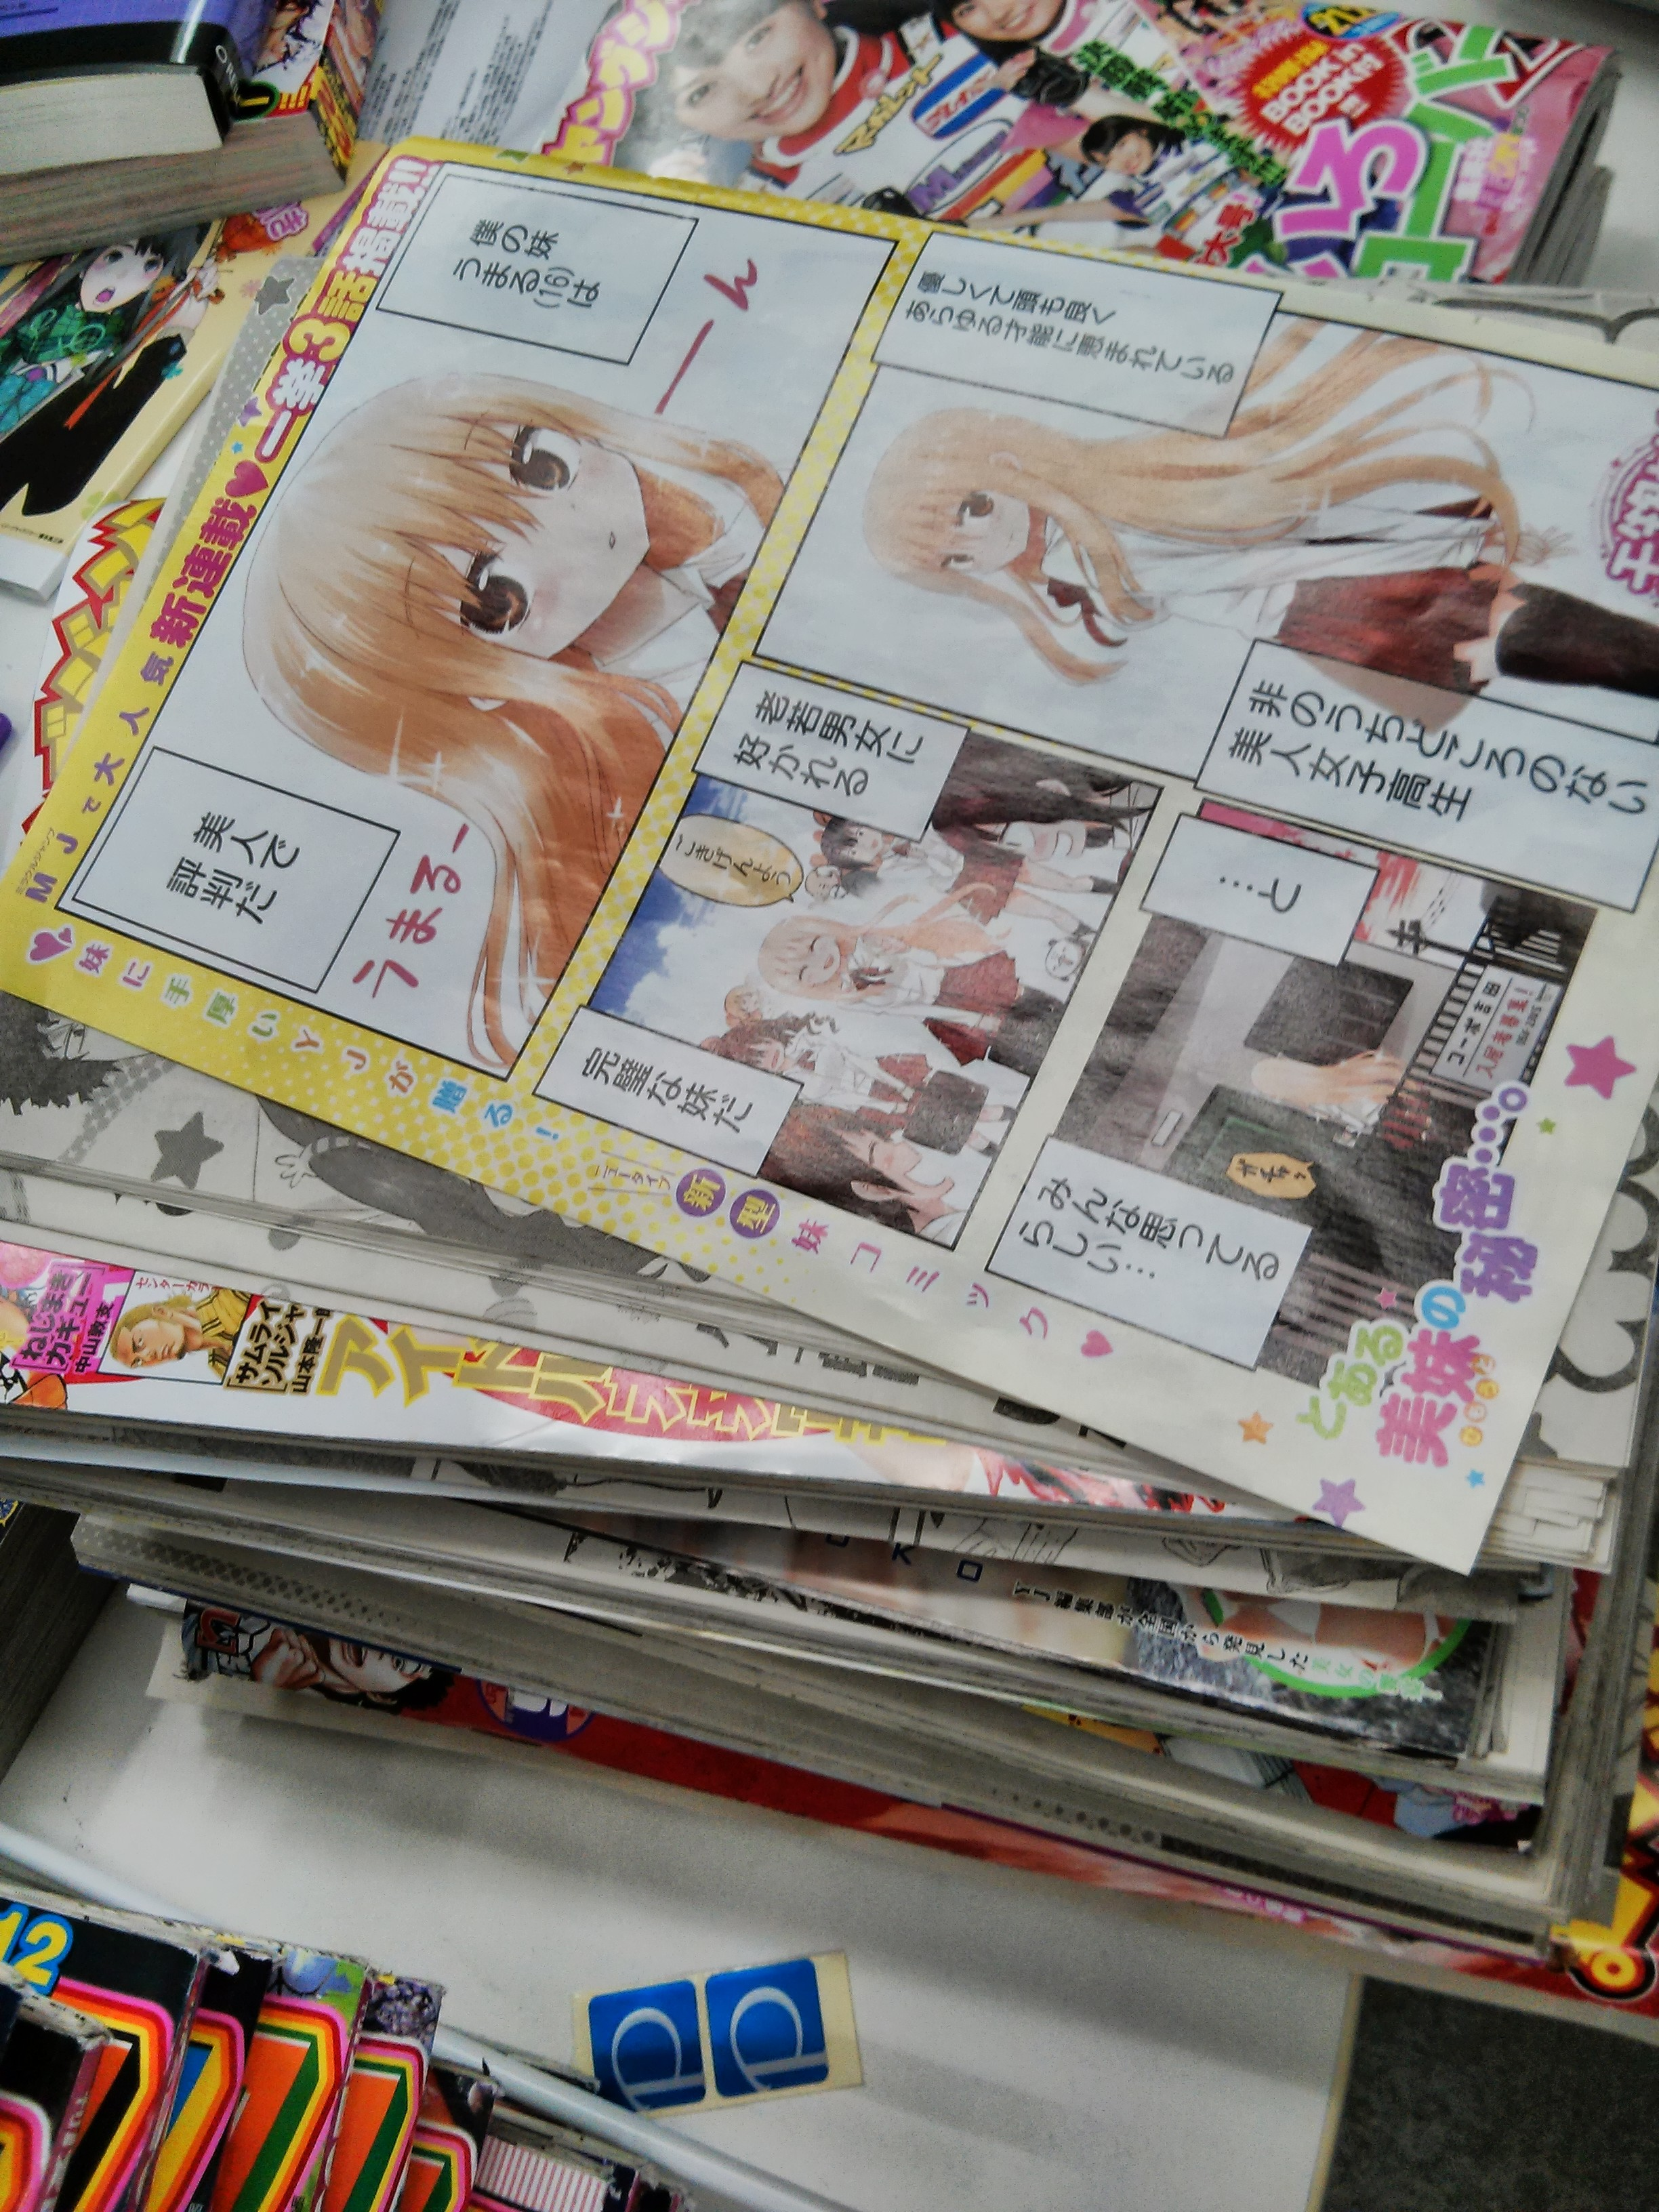
\includegraphics[width=0.4\textwidth]{../images/umaru.jpg}
  \caption{切り取られて手製単行本にされるうまるちゃん}
\end{figure}

\subsection{パターン2: 名前から言葉遊び}

機能の名前から言葉遊びでプロジェクト名を決める方法です。
これが一番訳のわからないプロジェクト名になって \emph{あとで困ります}

例えば \emph{Oauthプロバイダ} のプロジェクトは、 ``Oauth''
-\textgreater{} ``大須'' -\textgreater{} ``名古屋'' -\textgreater{}
``岸田メル先生'' -\textgreater{} ``ロロナのアトリエ'' と連想して最終的に
\emph{ロロナちゃん} になりました。
GitHub:Enterpriseの説明にもそう書いていますが、それを見ないともう由来がわからなくなっています。

Androidアプリのプロジェクト名は \emph{drosselお嬢様} ですが、
これが唯一わかりやすい (たぶん語源が一緒だし) 例だと言えます。

\subsection{パターン3: 機能の性質からキャラクター探し}

機能の性質からそれに適したキャラクターを探す方法です。
一番多い名付けパターンですが、名付けに一番時間がかかるパターンでもあります。

まずプロジェクトの持つ機能を「 \emph{人間にありそうな属性}
」に翻訳します。 ブレストのような感じでいくつも属性を出していきます。
その後、出てきた属性に当てはまりそうなキャラクターを延々と出し続けていきます。
読みやすさ、呼びやすさ、他のプロジェクトと混同しないかどうかなどを検討し、
\emph{しっくりきた} キャラクターがあらわれるまで繰り返します。

実際にそのキャラクターがしっくりくるかどうかは一瞬で判断でき、
すごく難産だったプロジェクト名でも、決まった瞬間は一瞬で全会一致した、という傾向があります。

属性にあったキャラクターを探すというのは、記憶をたどる作業なので、
ここで出てくるキャラクターは、 \emph{少し古いけど根強い人気がある}
キャラクターが多い傾向があります。
属性つながり、根強い人気、という観点から、最も親しまれるプロジェクトになるでしょう。
これなら偉い人に名前の理由を聞かれても答えやすいですよね。

例として

\begin{itemize}
\itemsep1pt\parskip0pt\parsep0pt
\item
  \emph{羽川さん} 書籍検索のSolrサーバ。『物語シリーズ』より。
  「何でもは知らないわ。インデックスされた書籍だけ。」
\item
  \emph{名雪さん} 朝会の時間と日直を知らせてくれるBOT。
  『Kanon』より。「朝ー朝だよー」 なお朝とは16時のことである。
\item
  \emph{めだかさん}
  全体的な要望とかを書き留めておくためのIssue用プロジェクト。『めだかボックス』の目安箱キャラということで。
\end{itemize}

みんな「さん」なのは何かの偶然

\subsection{パターン4: リアル嫁}

ニコ書チームでは、油断していると現実の嫁の名前もプロジェクト名にされます。

最初の例は、hogelogが担当する予定の書籍データ配信サーバを、 hogelogが(
\emph{結婚式で} )休んでいる隙を突いて、リーダーが独断で \emph{maki}
にしたのが始まりです。 この命名が不幸だったのは、 \emph{配信サーバ}
という性質から、同時接続数や転送速度の高い処理性能が求められ、
その性能要件を大幅に達成し全然余裕がある、という素晴らしい成果を達成したのに、
「maki、同時に何本も(接続を)咥えこんでやがるぜ」とか
「makiは(帯域がまだ)ガバガバだな」とか、
本人に向かっては絶対に言えない言葉で評価されたことでしょう。
偉い人に対しても「大丈夫です、makiガバガバなんで」みたいな言い方をしました。

2例目は、パターン3との複合事例で、件のリーダーの退職後に起こりました。
ちょうどその時、電子書籍が正しくコンバートされない問題が多発しており、
ファイルをチェックするプログラムが必要とされていました。
イメージで上がった「読書キャラ」から、『ハルヒ』の長門有希が連想されたけど、
yukiだとmakiとかぶるし、長門だと戦艦想像しちゃうし(
\emph{今なら問題ない} )と、却下しそうになった瞬間、
「イヤ、そうじゃなくて長門有希の
子音だけを抜き出し\footnote{https://twitter.com/ngtyk}て・・・」と言われ、
 その場にいた全員が「アッ」っと叫び「それだ!」と、
連想ゲームをしていたはずが、いつの間に件のリーダーのリアル嫁のプロジェクトができていました。

\subsection{まとめ}

可愛い女の子の名前をプロジェクト名にすると仕事のモチベーションがだいぶ違います。
何度も言いますが、偉い人の前でも堂々とこの呼び方をしましょう。
